\documentclass{standalone}
\usepackage{tikz}
\usetikzlibrary{patterns, positioning}


\begin{document}
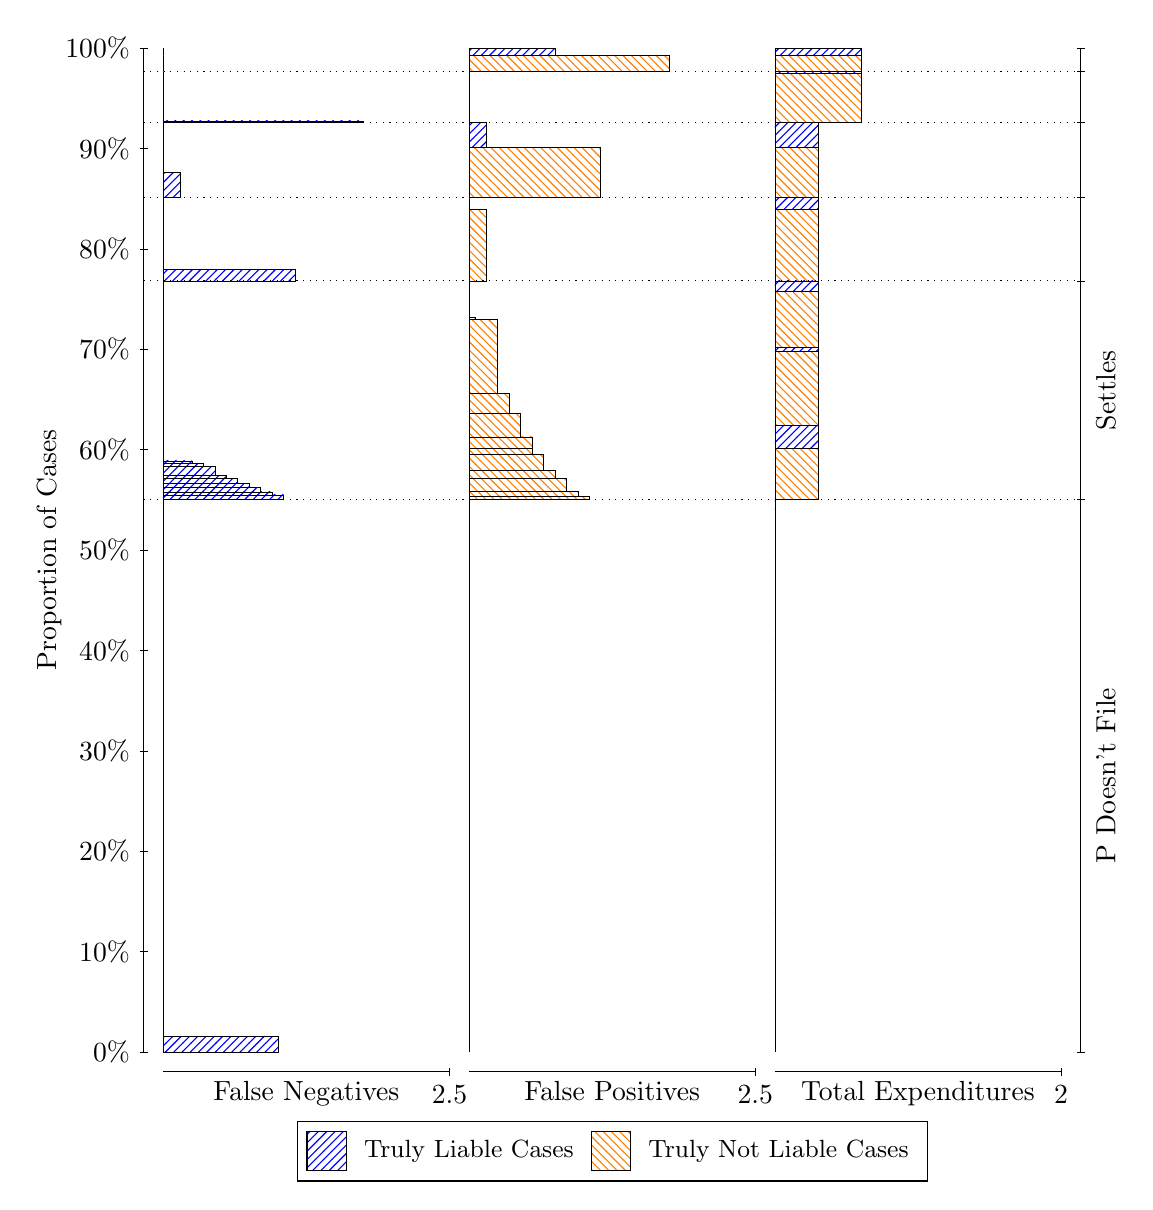
\begin{tikzpicture}
\draw[black, very thin] (1.5,1.75) -- (1.5,14.5);
\node[rotate=90, text=black, anchor=center] at (0.3, 8.125) {Proportion of Cases};
\draw[black, very thin] (1.45,1.75) -- (1.55,1.75);
\node[text=black, anchor=east] at (1.45, 1.75) {0\%};
\draw[black, very thin] (1.45,3.025) -- (1.55,3.025);
\node[text=black, anchor=east] at (1.45, 3.025) {10\%};
\draw[black, very thin] (1.45,4.3) -- (1.55,4.3);
\node[text=black, anchor=east] at (1.45, 4.3) {20\%};
\draw[black, very thin] (1.45,5.575) -- (1.55,5.575);
\node[text=black, anchor=east] at (1.45, 5.575) {30\%};
\draw[black, very thin] (1.45,6.85) -- (1.55,6.85);
\node[text=black, anchor=east] at (1.45, 6.85) {40\%};
\draw[black, very thin] (1.45,8.125) -- (1.55,8.125);
\node[text=black, anchor=east] at (1.45, 8.125) {50\%};
\draw[black, very thin] (1.45,9.4) -- (1.55,9.4);
\node[text=black, anchor=east] at (1.45, 9.4) {60\%};
\draw[black, very thin] (1.45,10.675) -- (1.55,10.675);
\node[text=black, anchor=east] at (1.45, 10.675) {70\%};
\draw[black, very thin] (1.45,11.95) -- (1.55,11.95);
\node[text=black, anchor=east] at (1.45, 11.95) {80\%};
\draw[black, very thin] (1.45,13.225) -- (1.55,13.225);
\node[text=black, anchor=east] at (1.45, 13.225) {90\%};
\draw[black, very thin] (1.45,14.5) -- (1.55,14.5);
\node[text=black, anchor=east] at (1.45, 14.5) {100\%};

\draw[black, very thin] (13.4,1.75) -- (13.4,14.5);
\draw[black, very thin] (13.35,1.75) -- (13.45,1.75);
\node[anchor=west] at (13.35, 1.75) {};
\draw[black, very thin] (13.35,8.7654) -- (13.45,8.7654);
\node[anchor=west] at (13.35, 8.7654) {};
\draw[black, very thin] (13.35,11.542) -- (13.45,11.542);
\node[anchor=west] at (13.35, 11.542) {};
\draw[black, very thin] (13.35,12.602) -- (13.45,12.602);
\node[anchor=west] at (13.35, 12.602) {};
\draw[black, very thin] (13.35,13.554) -- (13.45,13.554);
\node[anchor=west] at (13.35, 13.554) {};
\draw[black, very thin] (13.35,14.203) -- (13.45,14.203);
\node[anchor=west] at (13.35, 14.203) {};
\draw[black, very thin] (13.35,14.5) -- (13.45,14.5);
\node[anchor=west] at (13.35, 14.5) {};

\draw[black, very thin, pattern color=blue, pattern=north east lines] (1.75,1.75) rectangle (3.2033,1.9469);
\draw[black, very thin, pattern color=orange, pattern=north west lines] (1.75,1.9469) rectangle (1.75,8.7654);
\draw[black, very thin, pattern color=blue, pattern=north east lines] (1.75,8.7654) rectangle (3.276,8.8238);
\draw[black, very thin, pattern color=blue, pattern=north east lines] (1.75,8.8238) rectangle (3.1307,8.8636);
\draw[black, very thin, pattern color=blue, pattern=north east lines] (1.75,8.8636) rectangle (2.9853,8.9187);
\draw[black, very thin, pattern color=blue, pattern=north east lines] (1.75,8.9187) rectangle (2.84,8.9737);
\draw[black, very thin, pattern color=blue, pattern=north east lines] (1.75,8.9737) rectangle (2.6947,9.0341);
\draw[black, very thin, pattern color=blue, pattern=north east lines] (1.75,9.0341) rectangle (2.5493,9.0703);
\draw[black, very thin, pattern color=blue, pattern=north east lines] (1.75,9.0703) rectangle (2.404,9.1859);
\draw[black, very thin, pattern color=blue, pattern=north east lines] (1.75,9.1859) rectangle (2.2587,9.2295);
\draw[black, very thin, pattern color=blue, pattern=north east lines] (1.75,9.2295) rectangle (2.1133,9.2579);
\draw[black, very thin, pattern color=orange, pattern=north west lines] (1.75,9.2579) rectangle (1.75,11.542);
\draw[black, very thin, pattern color=blue, pattern=north east lines] (1.75,11.542) rectangle (3.4213,11.692);
\draw[black, very thin, pattern color=orange, pattern=north west lines] (1.75,11.692) rectangle (1.75,12.602);
\draw[black, very thin, pattern color=blue, pattern=north east lines] (1.75,12.602) rectangle (1.968,12.918);
\draw[black, very thin, pattern color=orange, pattern=north west lines] (1.75,12.918) rectangle (1.75,13.554);
\draw[black, very thin, pattern color=blue, pattern=north east lines] (1.75,13.554) rectangle (4.2933,13.576);
\draw[black, very thin, pattern color=orange, pattern=north west lines] (1.75,13.576) rectangle (1.75,14.203);
\draw[black, very thin, pattern color=orange, pattern=north west lines] (1.75,14.203) rectangle (1.75,14.402);
\draw[black, very thin, pattern color=blue, pattern=north east lines] (1.75,14.402) rectangle (1.75,14.5);
\draw[black, very thin, pattern color=orange, pattern=north west lines] (5.6333,1.75) rectangle (5.6333,8.5685);
\draw[black, very thin, pattern color=blue, pattern=north east lines] (5.6333,8.5685) rectangle (5.6333,8.7654);
\draw[black, very thin, pattern color=orange, pattern=north west lines] (5.6333,8.7654) rectangle (7.1593,8.8061);
\draw[black, very thin, pattern color=orange, pattern=north west lines] (5.6333,8.8061) rectangle (7.014,8.8694);
\draw[black, very thin, pattern color=orange, pattern=north west lines] (5.6333,8.8694) rectangle (6.8687,9.0391);
\draw[black, very thin, pattern color=orange, pattern=north west lines] (5.6333,9.0391) rectangle (6.7233,9.1321);
\draw[black, very thin, pattern color=orange, pattern=north west lines] (5.6333,9.1321) rectangle (6.578,9.3382);
\draw[black, very thin, pattern color=orange, pattern=north west lines] (5.6333,9.3382) rectangle (6.4327,9.4123);
\draw[black, very thin, pattern color=orange, pattern=north west lines] (5.6333,9.4123) rectangle (6.4327,9.5606);
\draw[black, very thin, pattern color=orange, pattern=north west lines] (5.6333,9.5606) rectangle (6.2873,9.8577);
\draw[black, very thin, pattern color=orange, pattern=north west lines] (5.6333,9.8577) rectangle (6.142,10.118);
\draw[black, very thin, pattern color=orange, pattern=north west lines] (5.6333,10.118) rectangle (5.9967,11.05);
\draw[black, very thin, pattern color=blue, pattern=north east lines] (5.6333,11.05) rectangle (5.706,11.078);
\draw[black, very thin, pattern color=blue, pattern=north east lines] (5.6333,11.078) rectangle (5.6333,11.542);
\draw[black, very thin, pattern color=orange, pattern=north west lines] (5.6333,11.542) rectangle (5.8513,12.453);
\draw[black, very thin, pattern color=blue, pattern=north east lines] (5.6333,12.453) rectangle (5.6333,12.602);
\draw[black, very thin, pattern color=orange, pattern=north west lines] (5.6333,12.602) rectangle (7.3047,13.237);
\draw[black, very thin, pattern color=blue, pattern=north east lines] (5.6333,13.237) rectangle (5.8513,13.554);
\draw[black, very thin, pattern color=orange, pattern=north west lines] (5.6333,13.554) rectangle (5.6333,14.181);
\draw[black, very thin, pattern color=blue, pattern=north east lines] (5.6333,14.181) rectangle (5.6333,14.203);
\draw[black, very thin, pattern color=orange, pattern=north west lines] (5.6333,14.203) rectangle (8.1767,14.402);
\draw[black, very thin, pattern color=blue, pattern=north east lines] (5.6333,14.402) rectangle (6.7233,14.5);
\draw[black, very thin, pattern color=orange, pattern=north west lines] (9.5167,1.75) rectangle (9.5167,8.5685);
\draw[black, very thin, pattern color=blue, pattern=north east lines] (9.5167,8.5685) rectangle (9.5167,8.7654);
\draw[black, very thin, pattern color=orange, pattern=north west lines] (9.5167,8.7654) rectangle (10.062,9.4123);
\draw[black, very thin, pattern color=blue, pattern=north east lines] (9.5167,9.4123) rectangle (10.062,9.7125);
\draw[black, very thin, pattern color=orange, pattern=north west lines] (9.5167,9.7125) rectangle (10.062,10.645);
\draw[black, very thin, pattern color=blue, pattern=north east lines] (9.5167,10.645) rectangle (10.062,10.703);
\draw[black, very thin, pattern color=orange, pattern=north west lines] (9.5167,10.703) rectangle (10.062,11.408);
\draw[black, very thin, pattern color=blue, pattern=north east lines] (9.5167,11.408) rectangle (10.062,11.542);
\draw[black, very thin, pattern color=orange, pattern=north west lines] (9.5167,11.542) rectangle (10.062,12.453);
\draw[black, very thin, pattern color=blue, pattern=north east lines] (9.5167,12.453) rectangle (10.062,12.602);
\draw[black, very thin, pattern color=orange, pattern=north west lines] (9.5167,12.602) rectangle (10.062,13.237);
\draw[black, very thin, pattern color=blue, pattern=north east lines] (9.5167,13.237) rectangle (10.062,13.554);
\draw[black, very thin, pattern color=orange, pattern=north west lines] (9.5167,13.554) rectangle (10.607,14.181);
\draw[black, very thin, pattern color=blue, pattern=north east lines] (9.5167,14.181) rectangle (10.607,14.203);
\draw[black, very thin, pattern color=orange, pattern=north west lines] (9.5167,14.203) rectangle (10.607,14.402);
\draw[black, very thin, pattern color=blue, pattern=north east lines] (9.5167,14.402) rectangle (10.607,14.5);
\draw[black, dotted] (1.5,8.7654) -- (13.4,8.7654);
\draw[black, dotted] (1.5,11.542) -- (13.4,11.542);
\draw[black, dotted] (1.5,12.602) -- (13.4,12.602);
\draw[black, dotted] (1.5,13.554) -- (13.4,13.554);
\draw[black, dotted] (1.5,14.203) -- (13.4,14.203);
\draw[black, very thin] (1.75,1.5) -- (5.3833,1.5);
\node[text=black, anchor=north] at (3.5667, 1.5) {False Negatives};
\draw[black, very thin] (5.3833,1.45) -- (5.3833,1.55);
\node[text=black, anchor=north] at (5.3833, 1.45) {2.5};

\draw[black, very thin] (5.6333,1.5) -- (9.2667,1.5);
\node[text=black, anchor=north] at (7.45, 1.5) {False Positives};
\draw[black, very thin] (9.2667,1.45) -- (9.2667,1.55);
\node[text=black, anchor=north] at (9.2667, 1.45) {2.5};

\draw[black, very thin] (9.5167,1.5) -- (13.15,1.5);
\node[text=black, anchor=north] at (11.333, 1.5) {Total Expenditures};
\draw[black, very thin] (13.15,1.45) -- (13.15,1.55);
\node[text=black, anchor=north] at (13.15, 1.45) {2};

\node[text=black, centered, rotate=90] at (13.72, 5.2577) {P Doesn't File};
\node[text=black, centered, rotate=90] at (13.72, 10.154) {Settles};





\draw (7.449999999999999,1.5) node[draw=none] (baseCoordinate) {};
\begin{scope}[align=center]
        \matrix[scale=0.5, draw=black, below=0.5cm of baseCoordinate, nodes={draw}, column sep=0.1cm]{
            \node[rectangle, draw, minimum width=0.5cm, minimum height=0.5cm, pattern color=blue, pattern=north east lines] {}; &
            \node[draw=none, font=\small, text=black] (B) {Truly Liable Cases}; &
            \node[rectangle, draw, minimum width=0.5cm, minimum height=0.5cm, pattern color=orange, pattern=north west lines] {}; &
            \node[draw=none, font=\small, text=black] (B) {Truly Not Liable Cases}; \\
            };
\end{scope}

\end{tikzpicture}
\end{document}